\documentclass{article}

% Configurações Genéricas ------------------------------------------------------
\usepackage[utf8]{inputenc}
\usepackage[T1]{fontenc}
\usepackage[brazil]{babel}
\usepackage{sbc-template}
\usepackage{graphicx}

% Informações Pessoais ---------------------------------------------------------
\title{Planejamento do Trabalho de Grau A}
\author{Wanderson Henrique Camargo Rosa\inst{1}}
\address{Programação para Dispositivos Móveis 2011/1\\Centro de Ciências Exatas
e Tecnológicas\\Universidade do Vale do Rio dos Sinos ---
UNISINOS\email{wandersonwhcr@gmail.com}}

% Documento --------------------------------------------------------------------
\begin{document}

\maketitle{}

% Apresentação -----------------------------------------------------------------
\section{Apresentação}
\label{sec:apresentacao}

Este documento tem como objeto apresentar o planejamento do trabalho de Grau A
desta disciplina. Durante o desenvolvimento, deverá ser implementado um
aplicativo Apresentador de \emph{Slides} sobre a plataforma Android.

Um Apresentador de \emph{Slides} é um dispositivo que permite o controle de
lâminas em apresentações, palestras ou seminários, à distância, sem a
necessidade de deslocamento até a máquina onde os documentos estão sendo
exibidos, fazendo com que o ministrante tenha uma melhor interação com o
público.

Este dispositivo é relativamente caro em comparação com as funcionalidades
simples disponíveis. Porém, podemos construir um programa sobre a Plataforma
Android que consegue suprir as mesmas necessidades.

O trabalho consiste em criar um aplicativo para Android que controle uma
apresentação de \emph{slides} utilizando Bluetooth ou Ethernet.

% Ferramentas ------------------------------------------------------------------
\section{Especificação}
\label{sec:especificacao}

Basicamente, este trabalho será dividido em duas fases distintas. Há a
necessidade primária de criação de um servidor que seja executado na
máquina local onde as lâminas estão sendo apresentadas, utilizando uma forma de
troca de dados com dispositivos externos. Através de um protocolo específico,
comandos podem ser transferidos à máquina local informando ações que podem ser
tomadas. Logo após, podemos criar um aplicativo sobre a Plataforma Android que
utilize este protocolo, informando estes possíveis comandos.

\subsection{Ferramentas}

O servidor será desenvolvido utilizando a linguagem de programação Java. Esta
linguagem foi escolhida devido a facilidade de utilização de \emph{streaming} de
dados e simulação de ações utilizando teclado. Também é facilitado o
desenvolvimento de uma \emph{interface} mais amigável. Não há como criar uma
conexão Bluetooth nativamente utilizando Java, portanto, deve ser utilizada a
biblioteca externa Bluecove.

Já o aplicativo cliente também será desenvolvido utilizando esta linguagem,
porém voltada para o Sistema Operacional Android. Em ambos os programas, o
ambiente de desenvolvimento será Eclipse. Testes serão feitos utilizando
emulador disponível e um Samsung Galaxy 5 GT-I5500B com Sistema Operacional
Android 2.2 Froyo como dispositivo físico.

% Abstração de Elementos -------------------------------------------------------
\section{Abstração de Elementos}
\label{sec:abstracao}

Primeiramente, podemos criar diagramas de classe de alto nível para descrever a
estrutura que deve ser implementada. O programa servidor e o aplicativo cliente
estão descritos abaixo.

\subsection{Serviço}

O serviço de conexão na máquina local pode ser desenvolvido separadamente do
interpretador local de comandos enviados pelo dispositivo externo. Portanto,
haverá uma divisão entre tratamento de conexões e processamento destes comandos.

Isto torna possível a criação de qualquer programa que utilize as informações
enviadas de uma forma mais simples, já que as regras de conexão estarão
separadas e encapsuladas. Adicionalmente, uma camada de visualização será criada
isoladamente utilizando uma referência do interpretador.

\begin{figure}
    \centering{}
    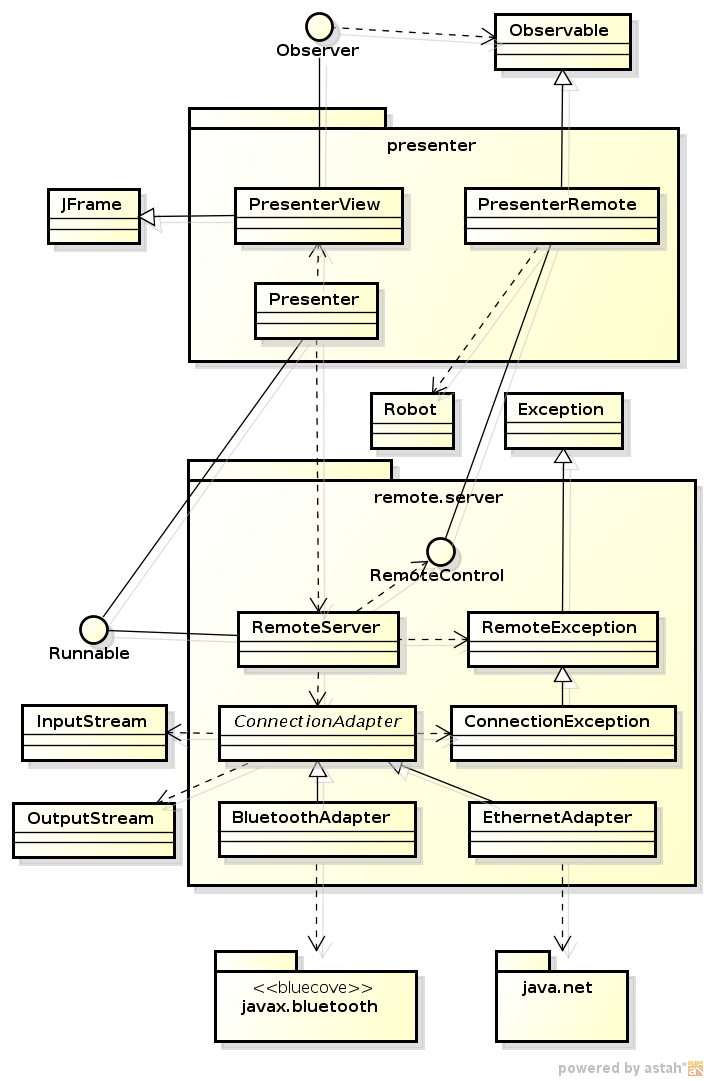
\includegraphics[scale=0.65]{presenter-server.png}
    \caption{Diagrama de Classes do Servidor}
    \label{fig:server}
\end{figure}

As regras de conexão são diferenciadas dependendo do \emph{hardware} de
transferência. Podemos criar uma classe abstrata que defina os principais
métodos, onde especializações deverão ser implementadas para cada um destes
tipos. Neste caso, há a necessidade adaptadores para conexão por Bluetooth ou
Ethernet. Por fim, devemos utilizar uma classe do Java que pode simular tarefas
do usuário, como pressionar teclas ou movimentação de \emph{mouse}.

Todas estas estruturas estão descritas na Figura \ref{fig:server}.
Como podemos visualizar, estão sendo utilizados os padrões de projeto Adapter
para criar a abstração de conexão e Observer para troca de informações entre
camadas de visualização e transferência de dados.

\subsection{Cliente}

O aplicativo cliente deve receber a mesma estrutura para conexão com
adaptadores. O Sistema Operacional Android utiliza atividades como elementos
principais de programação. Portanto, teremos uma atividade que exibe os arquivos
de ajuda ao usuário e outra para configurações globais do aplicativo.

\subsubsection{Listagem de Elementos}

Há uma atividade principal que deve listar todos os dispositivos cadastrados no
sistema, incluindo Bluetooth e Ethernet. Dispositivos Bluetooth devem ser
administrados pela atividade de configurações Bluetooth, padrão do Android. Já a
conexão por Ethernet somente é possível caso um dispositivo deste tipo seja
adicionado no aplicativo. Os elementos listados nesta atividade podem ser
removidos; por isso, todos devem armazenar informações em banco de dados local.
A listagem de elementos será decrescente conforme horário da última conexão.

\subsubsection{Banco de Dados}

Centralizando o acesso ao banco, deve ser incluida uma classe representante de
aplicativos Android, onde devemos adicionar uma nova referência para a conexão
de dados, trabalhando como um padrão de projeto Singleton. A atividade que
controla a apresentação é responsável por toda a manipulação de dados para
comunicação. Esta estrutura pode ser visualizada em diagrama de classe, conforme
Figura \ref{fig:client}.

\begin{figure}
    \centering{}
    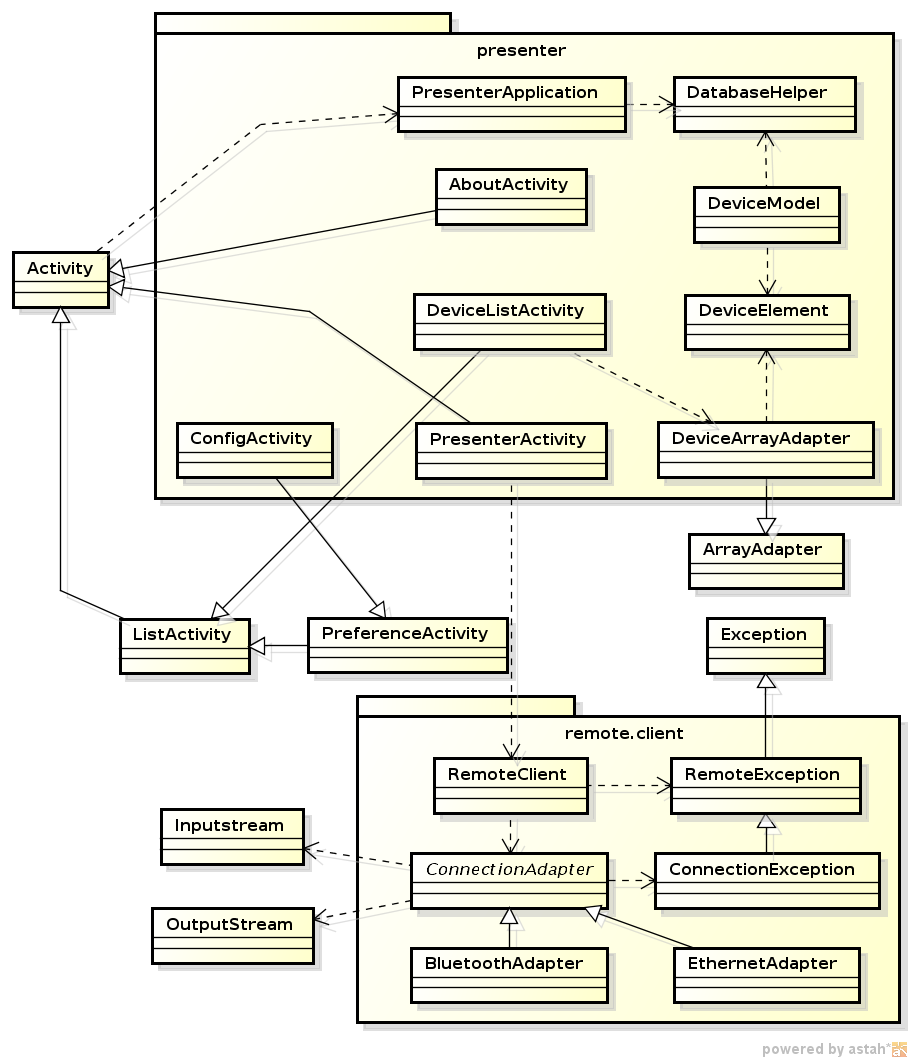
\includegraphics[width=\textwidth]{presenter-client.png}
    \caption{Diagrama de Classes Cliente}
    \label{fig:client}
\end{figure}

\subsection{Visualização Serviço}

Utilizando a estrutura do serviço, deve ser implementada uma pequena
\emph{interface} para controle da apresentação de \emph{slides}, conforme a
Figura \ref{fig:server-view}.

\begin{figure}
    \centering{}
    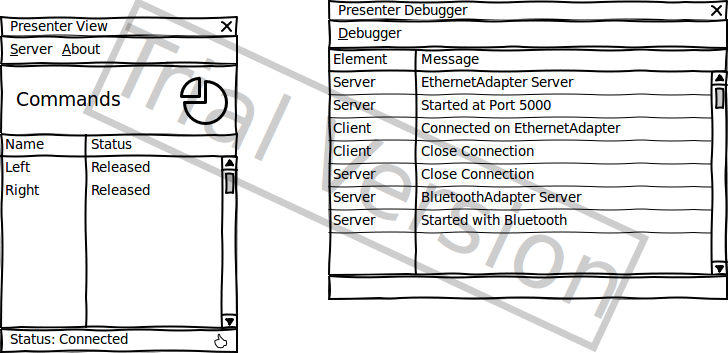
\includegraphics[scale=0.55]{presenter-server-view.png}
    \caption{\emph{Interface} do Servidor}
    \label{fig:server-view}
\end{figure}

A janela principal deve apresentar todos os possíveis comandos que podem ser
utilizados pelo Apresentador de \emph{Slides} e o estado da ação de cada um
deles. Também deve estar visível o estado do serviço.

O usuário pode solicitar a verificação de mensagens registradas pelo servidor
em tempo de execução. Cada linha deve ser identificada pelo dispositivo que
executou a ação, seguido de uma mensagem do sistema.

\subsection{Visualização Cliente}

A \emph{interface} no Android deve ser semelhante ao exemplo desenvolvido na
Figura \ref{fig:client-view}. Existe uma listagem de todos os dispositivos
cadastrados no Sistema e que podem ser gerenciados. Também há necessidade de
criação de um menu de contexto para acesso a outras atividades do aplicativo.

\begin{figure}
    \centering{}
    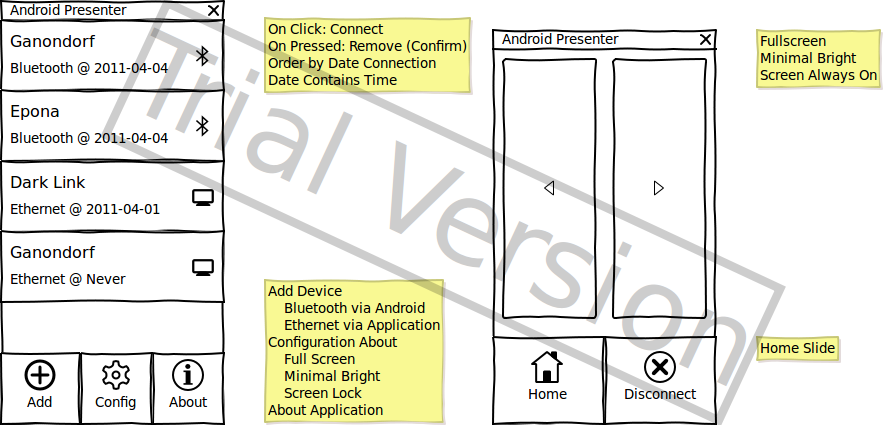
\includegraphics[width=\textwidth]{presenter-client-view.png}
    \caption{\emph{Interface} do Cliente}
    \label{fig:client-view}
\end{figure}

A tela do Apresentador basicamente possui dois botões que devem executar a
movimentação das lâminas para a frente ou para trás. No menu de contexto é
possível ir para a página inicial do documento utilizando um botão específico.

\subsubsection{Preferências}

Deve ser implementada uma atividade para cadastro de preferências do usuário,
como exibição do aplicativo em tela cheia, redução de brilho para economia de
bateria ou para evitar que o dispositivo fique bloqueado quando não utilizado
durante as apresentações.

% Protocolo --------------------------------------------------------------------
\section{Protocolo}
\label{sec:protocolo}

A transferência de comandos entre o dispositivo e a máquina local será feita
utilizando um protocolo baseado em notação de objetos em Javascript (JSON). Esta
sequência de caracteres simboliza um objeto que pode ser construído em tempo de
execução e tratados como comandos no servidor. Para a escolha da estrutura
utilizada pelo protocolo, foram analisadas três tipos de notações: binária, XML
e JSON.

Utilizando um tratamento binário, a transferência de comandos seria otimizada,
porém o desenvolvimento de novas aplicações se tornaria mais complicado, fugindo
muito da forma humana de interpretação. A marcação XML tornaria o tratamento
dos comandos muito mais simples, porém a transferência perderá velocidade devido
a quantidade de caracteres adicionais.

Entre estas duas necessidades, o JSON aparentou ser de fácil interpretação,
visível numa forma mais humana e com quantidade menor de caracteres adicionais
durante a transferência.

A camada de interpretação das instruções deve ser desenvolvida no servidor,
separadamente da lógica de comunicação entre dispositivo móvel e máquina local,
utilizando um objeto que implemente a \emph{interface} de controle, conforme
diagrama da Figura \ref{fig:server}.

% Considerações Finais ---------------------------------------------------------
\section{Considerações Finais}
\label{sec:finais}

O projeto de comunicação entre um dispositivo móvel e máquina local pode crescer
ainda mais. Como houve uma preocupação em divisões entre comunicação, tratamento
de dados transferidos e visualização, será possível criar qualquer aplicativo
que utilize este tipo de serviço.

Podemos exemplificar com a modificação dos dados na transferência, onde sejam
informados os valores de posicionamento e sensores de acelerômetro do
dispositivo móvel, utilizando o mesmo protocolo. O objeto de tratamento pode ser
customizado para que identifique estes novos valores e interprete os movimentos
do usuário, executando comandos na máquina local. Neste caso, como há divisão de
responsabilidade, a visualização não precisa ser modificada.

Logo, este serviço poderá ser tratado como um motor de comunicação e pode ser
utilizado em inúmeras áreas e em dispositivos móveis variados, desde que
comuniquem-se com o mesmo protocolo. Inclusive podemos criar um cliente que seja
executado em outra máquina, transmita os comandos necessários e navegue nas
apresentações.

Após a finalização deste trabalho, o motor de comunicação será utilizado para os
próximos projetos, principalmente para o tratamento de valores de acelerômetro
informados pelo dispositivo móvel, controlando a apresentação de \emph{slides}
ou qualquer tipo de movimentação remota, como ambientes virtuais.

\end{document}